\section{Experiments}

\subsection{Experiment Setup}
The training process of RWKV-X consists of two stages: alignment pretraining and long-context continual pretraining. In the alignment pretraining stage, the RWKV-7 blocks are frozen, with only the Sparse Attention blocks being updated. During the long context continual pretraining stage, we finetune all parameters. Details of training data and hyper-parameters can be found in Appendix \ref{sec:data_Hyperparameters}.

\subsection{Long Context Evaluation}
To better understand the long-context capabilities of RWKV-X, we conduct a case study using the Single Needle-In-A-Haystack (S-NIAH) benchmark suite from RULER~\citep{hsieh2024rulerwhatsrealcontext}, where a key-value pair is embedded within a long context and the model is required to retrieve the value when given the corresponding key. 
The results are summarized in Table~\ref{tab:S-NIAH}, with some values sourced from the Gated DeltaNet paper~\cite{yang2024gated}.

\begin{table*}[h]
\centering
\caption{Zero-shot Performance Comparison on the S-NIAH Benchmark: S-NIAH-1 (Pass-key Retrieval), S-NIAH-2 (Number in Haystack), and S-NIAH-3 (UUID in Haystack).}
\label{tab:S-NIAH}
\resizebox{\textwidth}{!}
{
\begin{tabular}{l|cccc|cccc|cccc}
\toprule
\textbf{Model} & \multicolumn{4}{c|}{\textbf{S-NIAH-1}} & \multicolumn{4}{c|}{\textbf{S-NIAH-2}} & \multicolumn{4}{c}{\textbf{S-NIAH-3}} \\
& 1K & 2K & 4K & 8K & 1K & 2K & 4K & 8K & 1K & 2K & 4K & 8K \\
\midrule
RWKV-7-0.19B & 100 & 100 & 100 & 100 & 100 & 98.4 & 5.2 & 3.2 & 98.4 & 96.8 & 27.6 & 6.6 \\
RWKV-X-0.22B & 100 & 100 & 100 & 100 & 100 & 99.6 & 18.8 & 3.6 & 99.0 & 92.6 & 40.2 & 1.6 \\
\midrule
DeltaNet-1.3B & 97.4 & 96.8 & 99.0 & 98.8 & 98.4 & 45.6 & 18.6 & 14.4 & 85.2 & 47.0 & 22.4 & - \\
Mamba2-1.3B & 99.2 & 98.8 & 65.4 & 30.4 & 99.4 & 98.8 & 56.2 & 17.0 & 64.4 & 47.6 & 4.6 & - \\
Gated DeltaNet-1.3B & 98.4 & 88.4 & 91.4 & 91.8 & 100.0 & 99.8 & 92.2 & 29.6 & 86.6 & 84.2 & 27.6 & - \\
RWKV-6-1.6B & - & - & 98.0 & - & - & - & 53.0 & - & - & - & 55.0 & - \\
\midrule
RWKV-6-3B & - & - & 100 & - & - & - & 88.0 & - & - & - & 79.0 & - \\
RWKV-7-2.9B & - & - & 100 & - & - & - & 88.0 & - & - & - & 79.0 & - \\
\textbf{RWKV-X-3.6B} & \textbf{100} & \textbf{100} & \textbf{100} & \textbf{100} & \textbf{100} & \textbf{100} & \textbf{100} & \textbf{99.8} & \textbf{100} & \textbf{100} & \textbf{99.8} & \textbf{95.6} \\
\bottomrule
\end{tabular}
}
\end{table*}

\subsection{Short Context Evaluation}

Table~\ref{tab:short_context_benchmarks} presents the performance of RWKV-X across a range of short-context language understanding benchmarks, in comparison with prior RWKV variants and several strong baselines of similar or larger scale.
Among small-scale models, RWKV-X (0.22B) achieves an average score of 51.0, which is competitive with RWKV-7 (51.8).
In the large-scale regime, RWKV-X (3.6B) achieves an average score of 71.9, closely matching the performance of RWKV-7 (2.9B, 72.8) and Qwen2.5-3B (71.4), while outperforming LLaMA3.2-3B (69.7). 
These results demonstrate that RWKV-X maintains high performance on short-context tasks while offering architectural benefits for long-context modeling, confirming its effectiveness as a general-purpose LLM backbone.

\begin{table*}[htbp]
\centering
\caption{Evaluation results on short-context benchmarks, including LAMBADA, HellaSwag, PIQA, ARC-Easy (arcE), ARC-Challenge (arcC), Winogrande, SciQ, and MMLU.}
\label{tab:short_context_benchmarks}
\resizebox{\textwidth}{!}{%
\begin{tabular}{lrcccccccccc}
\toprule
\textbf{Model} & \textbf{Tokens} & \textbf{LAMBADA} & \textbf{HellaSwag} & \textbf{PIQA} & \textbf{arcE} & \textbf{arcC} & \textbf{Winogrande} & \textbf{SciQ} & \textbf{MMLU} & \textbf{avg} \\
(Name) & (T) & acc$\uparrow$ & acc\_n$\uparrow$ & acc$\uparrow$ & acc$\uparrow$ & acc$\uparrow$ & acc$\uparrow$ & acc$\uparrow$ & acc$\uparrow$ & acc$\uparrow$ \\
\midrule
RWKV-5-0.19B & 0.6 & 38.4 & 31.9 & 61.4 & 44.2 & 19.9 & 52.9 & 76.3 & 23.1 & 43.5 \\
SmoLLM2-135M & 2.0 & 42.9 & 43.1 & 68.1 & 64.4 & 28.1 & 53.4 & 80.1 & 25.8 & 50.7 \\
RWKV-7-0.19B & 1.6 & 48.1 & 42.1 & 67.3 & 59.3 & 25.5 & 56.0 & 86.3 & 30.1 & 51.8 \\
RWKV-X 0.22B & 1.6 & 47.0 & 42.1 & 67.9 & 56.9 & 29.4 & 52.6 & 86.1 & 26.0 & 51.0 \\
\midrule
RWKV-6-3B & 2.5 & 71.7 & 68.4 & 76.4 & 71.2 & 35.6 & 66.3 & 92.2 & 28.3 & 63.8 \\
Llama3.2-3B & 15.0 & 70.5 & 73.6 & 76.7 & 74.5 & 42.2 & 68.2 & 95.6 & 56.5 & 69.7 \\
Qwen2.5-3B & 18.0 & 67.1 & 73.5 & 77.4 & 77.1 & 45.0 & 68.8 & 96.2 & 65.7 & 71.4 \\
RWKV-7-2.9B & 5.6 & 73.4 & 76.4 & 79.7 & 81.0 & 48.7 & 72.8 & 95.0 & 55.0 & 72.8 \\
RWKV-X 3.6B & 5.6 & 73.1 & 74.5 & 79.4 & 80.0 & 50.6 & 70.6 & 95.0 & 52.3 & 71.9 \\
\bottomrule
\end{tabular}%
}
\end{table*}


\begin{figure}[tbp]
    \centering
    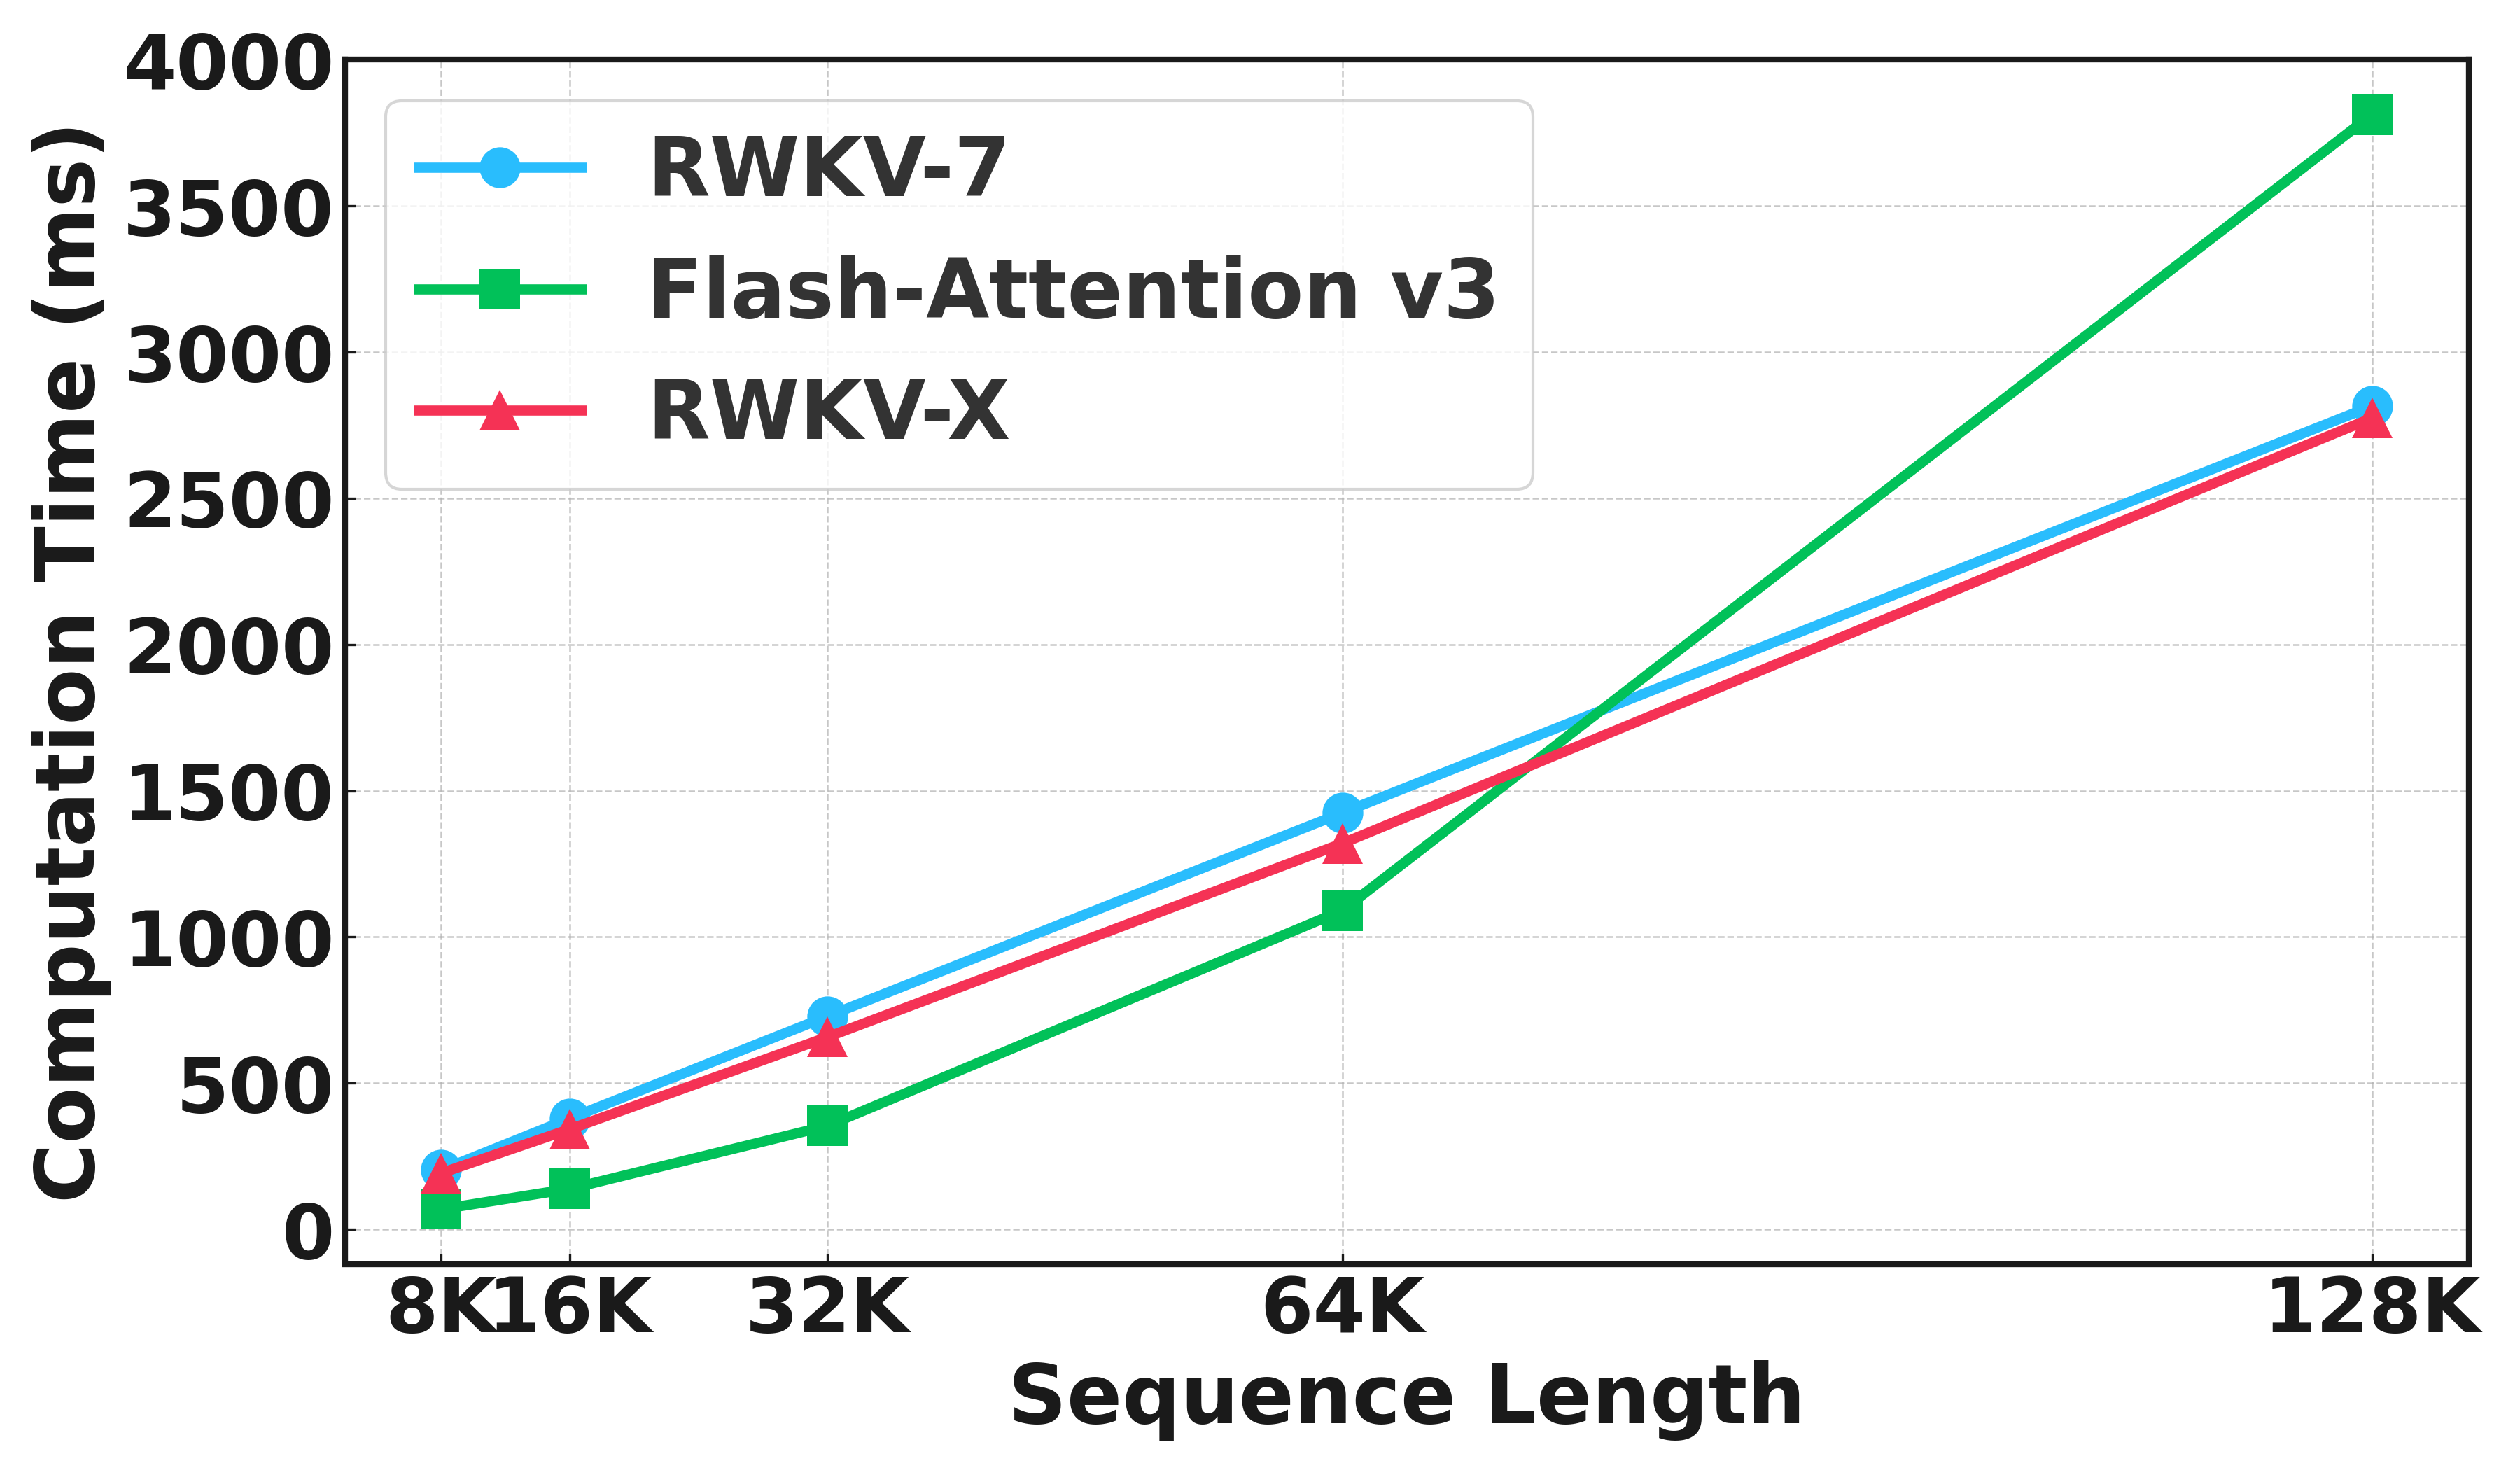
\includegraphics[width=\columnwidth]{figures/infer_efficiency.png}
    \caption{Prefill latency comparison between RWKV-X and a full-attention Transformer.}
    \label{fig:efficiency_comparison}
\end{figure}

\subsection{Efficiency Analysis}

Figure ~\ref{fig:efficiency_comparison} presents a comparison of prefill latency across different sequence lengths for RWKV-X, RWKV-7, and a full-attention Transformer using Flash-Attention v3~\cite{Shah2024FlashAttention3FA}. 
While Flash-Attention v3 demonstrates the lowest latency at shorter sequence lengths (8K–16K), its computation time increases steeply for longer inputs due to its quadratic complexity. 
At 128K, RWKV-X achieves a 1.37× speedup over Flash-Attention v3. Moreover, this speedup is expected to further improve as the input context length increases. 
RWKV-X exhibits near-linear scaling and consistently outperforms or matches RWKV-7, highlighting its superior efficiency and scalability for long-context inference.

The results in Figure~\ref{fig:rwkvx-latency} highlight the efficiency of RWKV-X-3.6B in handling long-context decoding. 
Despite RWKV-7-2.9B achieving lower absolute latency, RWKV-X-3.6B demonstrates remarkable stability across increasing context lengths, maintaining consistent decoding times even at 1M tokens. 
RWKV-X-3.6B employs a fixed 64K KV cache, while RWKV-7-2.9B operates without additional caching mechanisms.
RWKV-X demonstrates stable decoding latency as the context length increases.

\begin{figure}[tbp]
    \centering
    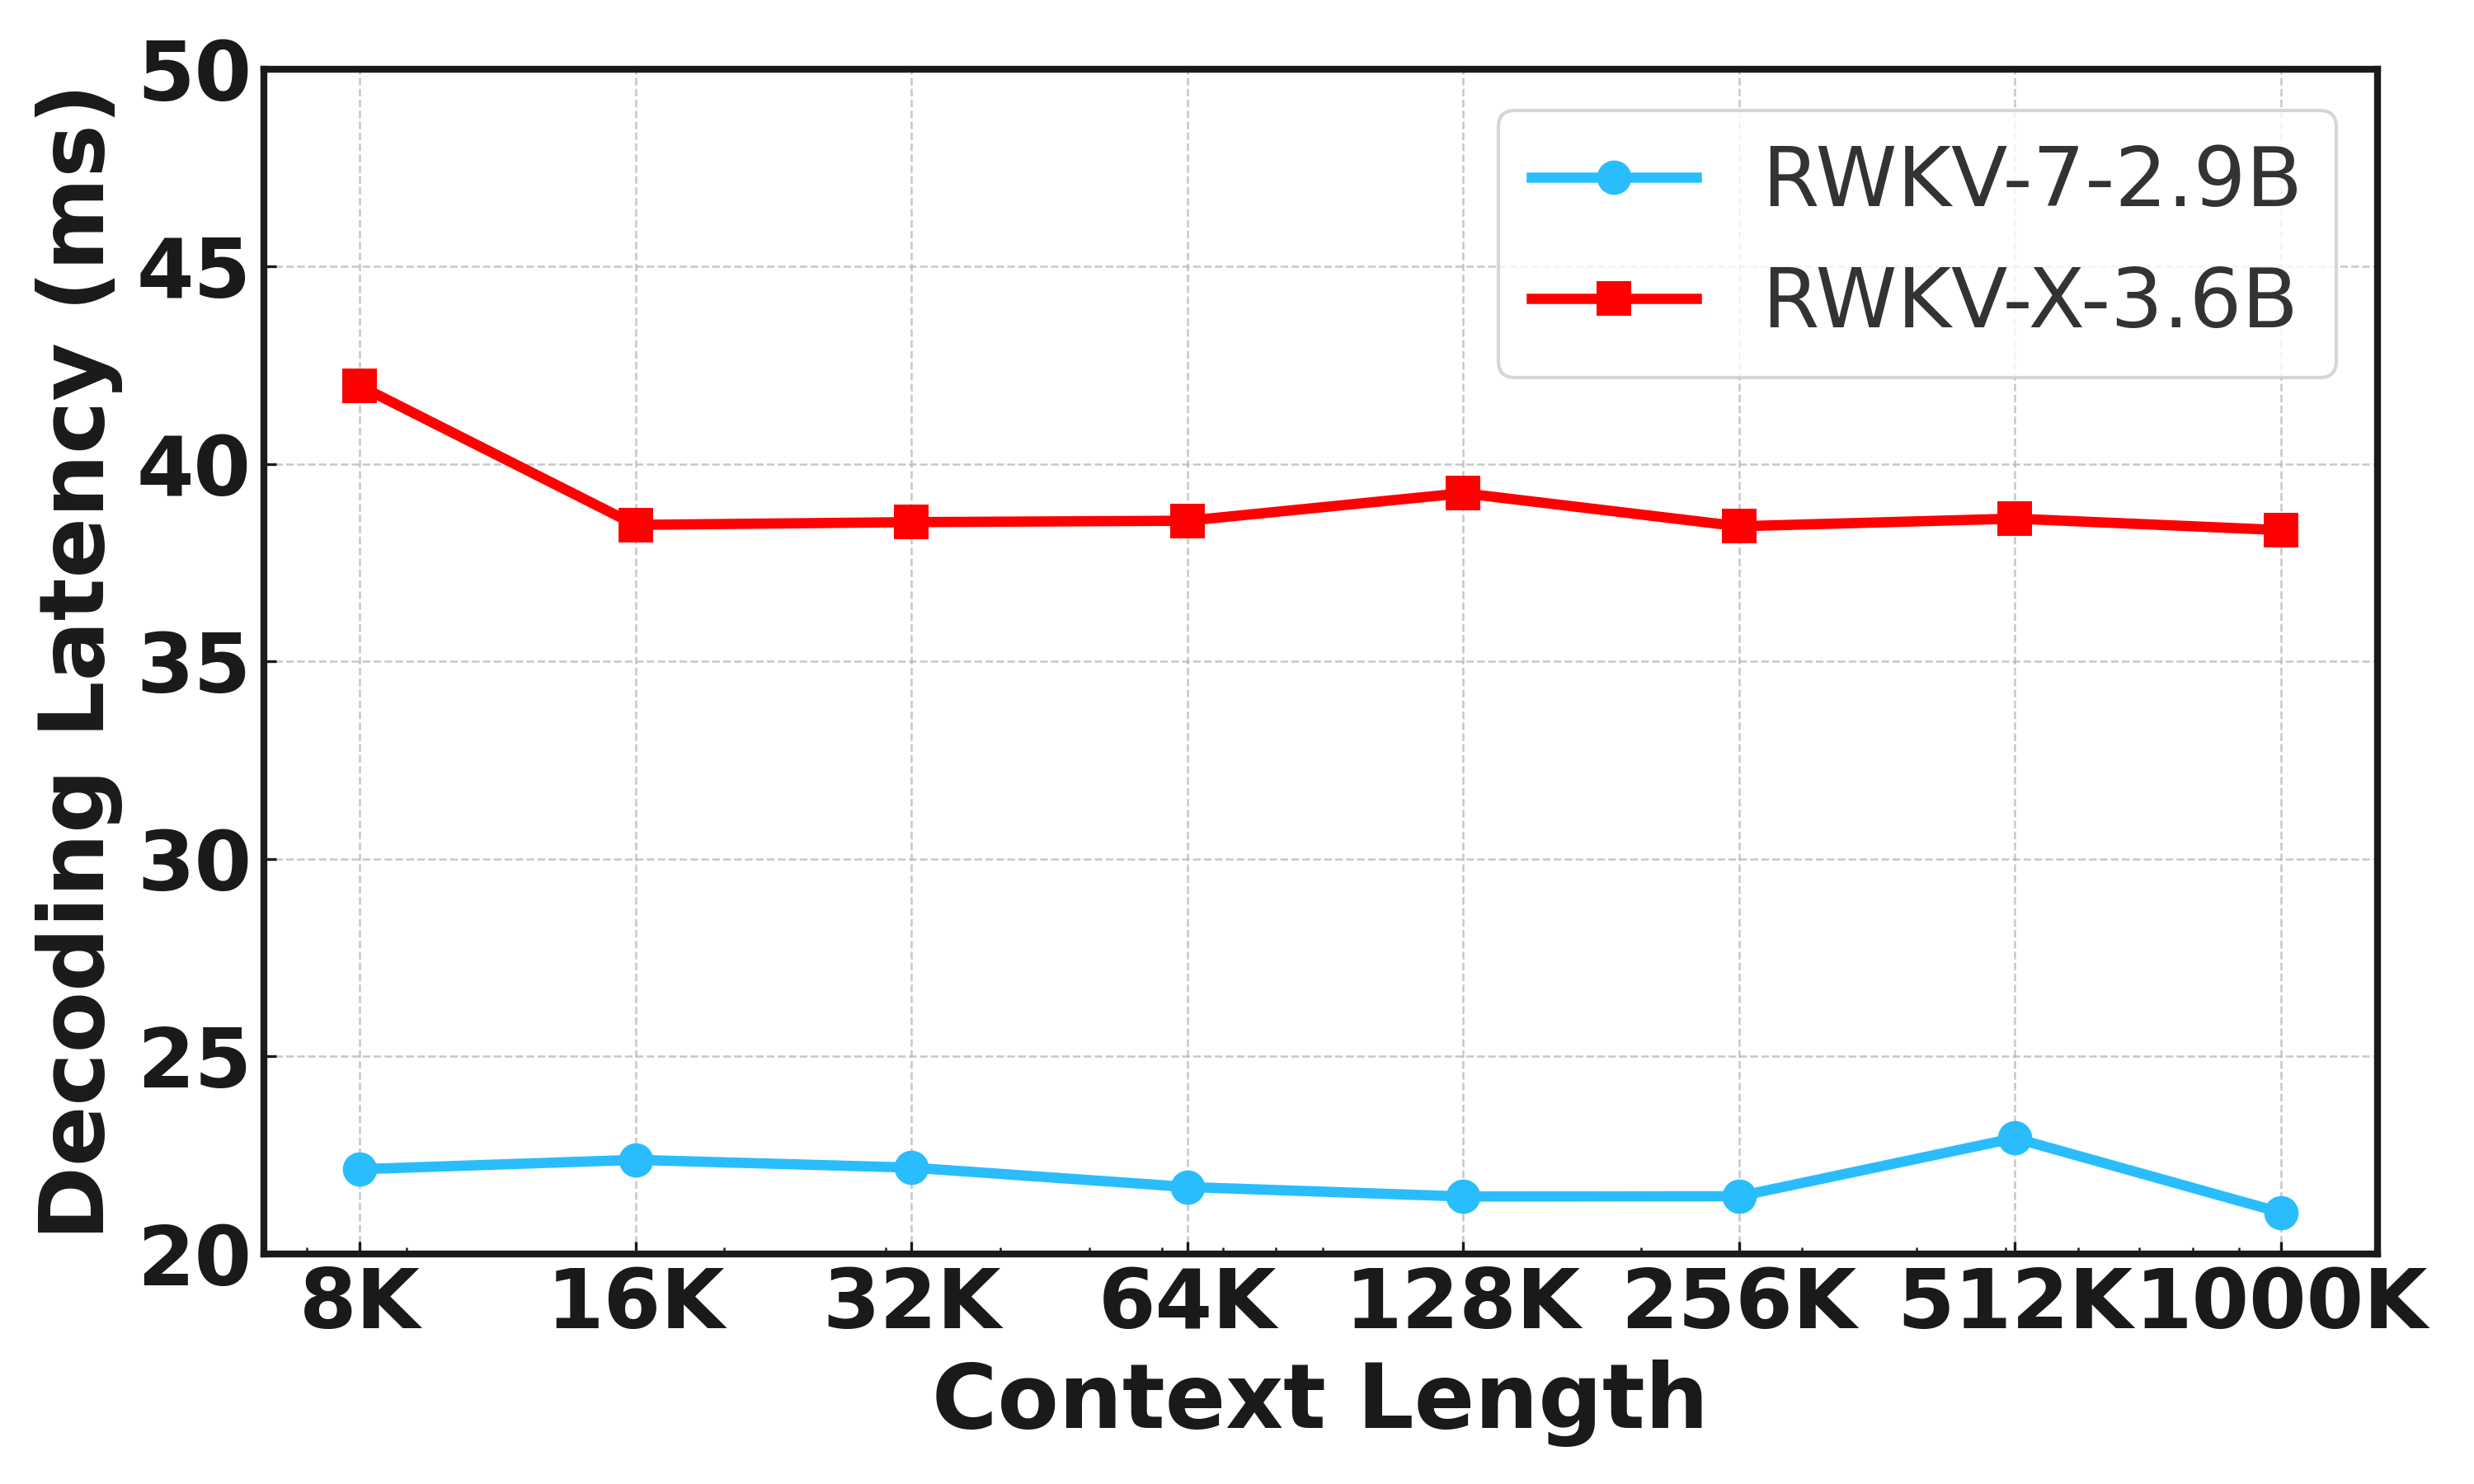
\includegraphics[width=\columnwidth]{figures/decoding_latency.png}
    \caption{Decoding latency comparison between RWKV-7-2.9B and RWKV-X-3.6B models.
    The horizontal axis represents the context length (log scale).}
    \label{fig:rwkvx-latency}
\end{figure}

\subsection{Ablation Study}

\subsubsection{Ablation on Long context Cross Entropy}

We conduct an ablation study to evaluate the impact of the Long-context Cross-Entropy~(LongCE) loss on the performance of RWKV-X-3.6B across three tasks in the S-NIAH benchmark. As shown in Table~\ref{tab:longce_ablation}, incorporating LongCE consistently improves model performance, particularly on tasks that require longer context understanding.

On S-NIAH-1, where the task involves relatively short-context retrieval, both versions of the model— with and without LongCE—achieve perfect accuracy across all context lengths, indicating that LongCE has minimal impact when the contextual challenge is low.

However, for S-NIAH-2 and S-NIAH-3, which demand deeper reasoning over longer input sequences, the benefits of LongCE become evident. At 8K context length, the model without LongCE shows a steep drop in performance—falling to 67.0 on S-NIAH-2 and 62.6 on S-NIAH-3. In contrast, the full model with LongCE maintains high accuracy at 99.8 and 95.6, respectively. These results demonstrate that LongCE plays a crucial role in helping the model focus on semantically important tokens over extended contexts, thereby preserving performance as sequence length increases.

Overall, LongCE significantly enhances the long-context generalization ability of RWKV-X, especially in tasks where key information is sparsely distributed across the input.

\begin{table}[h]
\centering
\caption{Ablation Study on LongCE Loss using the S-NIAH Benchmark (Higher is Better).}
\label{tab:longce_ablation}
\resizebox{\linewidth}{!}{
\begin{tabular}{llcccc}
\toprule
\textbf{Model} & \textbf{Task} & \textbf{1K} & \textbf{2K} & \textbf{4K} & \textbf{8K} \\
\midrule
RWKV-X-3.6B      & S-NIAH-1 & 100.0 & 100.0 & 100.0 & 100.0 \\
w/o LongCE       & S-NIAH-1 & 100.0 & 100.0 & 100.0 & 100.0 \\
\midrule
RWKV-X-3.6B      & S-NIAH-2 & 100.0 & 100.0 & 100.0 & \textbf{99.8} \\
w/o LongCE       & S-NIAH-2 & 100.0 & 100.0 & 98.4  & 67.0 \\
\midrule
RWKV-X-3.6B      & S-NIAH-3 & 100.0 & 100.0 & 99.8  & \textbf{95.6} \\
w/o LongCE       & S-NIAH-3 & 100.0 & 100.0 & 98.4  & 62.6 \\
\bottomrule
\end{tabular}
}
\end{table}

\subsubsection{Ablation on Percentage of Attention Layers}

We begin by investigating how the number of Sparse Attention layers affects model performance in RWKV-X. 
In this study, we train 126M-parameter hybrid models with 12 total layers, varying the proportion of Sparse Attention layers while distributing them evenly throughout the model. Figure~\ref{fig:val_loss_vs_attention_percentage} reports the validation loss as a function of the attention layer ratio, where 0\% corresponds to RWKV-7 and 100\% corresponds to a fully Sparse-Attention Transformer.
Our results show that validation loss is minimized when approximately 25\% of the layers are Sparse Attention layers. 
This suggests that a hybrid architecture offers advantages over both the pure RWKV-7 and the fully attention-based Transformer in terms of loss.

\begin{figure}[htbp]
    \centering
    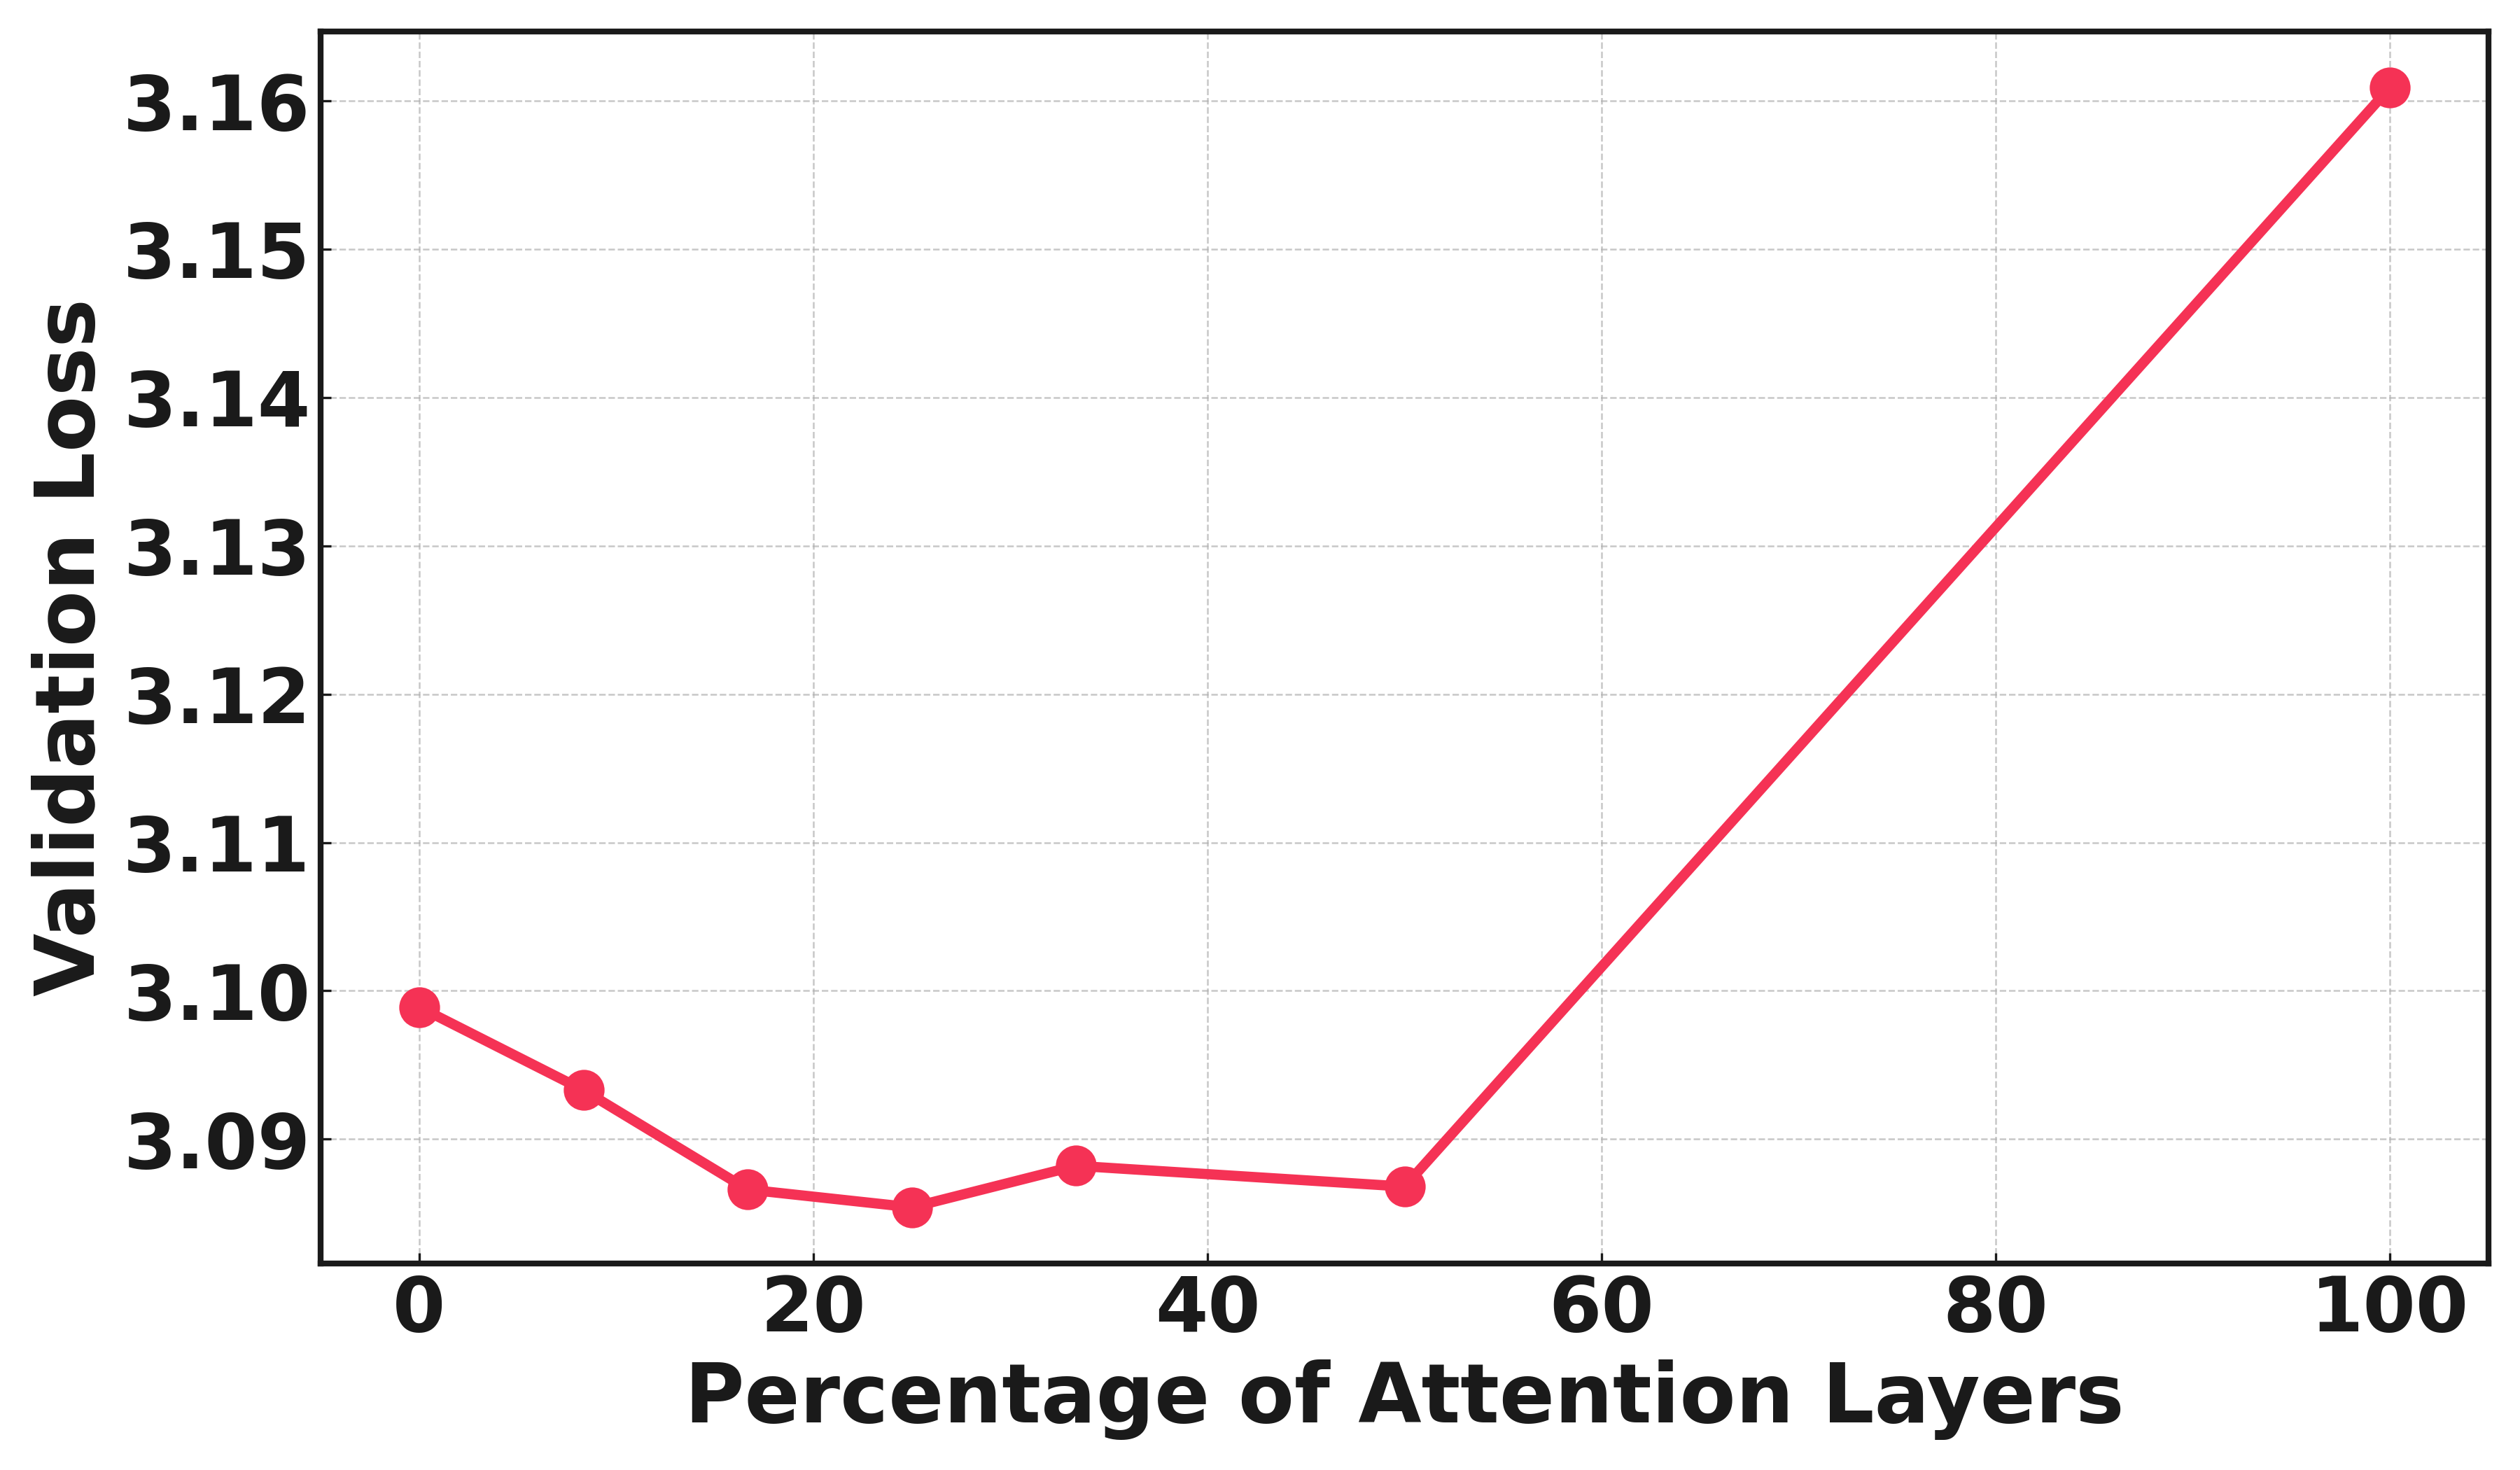
\includegraphics[width=\columnwidth]{figures/val_loss_vs_attention_percentage.png}
    \caption{Validation loss vs. percentage of attention layers for 124M-parameter RWKV-X models (12 layers). 0\% = RWKV-7, 100\% = Fully Sparse-Attention Transformer.}
    \label{fig:val_loss_vs_attention_percentage}
\end{figure}


\subsubsection{Ablation on Model Size}

Table~\ref{tab:perplexity_tokens} presents the validation loss comparison between GPT-2~\footnote{Code: https://github.com/xforcevesa/mixed-nanogpt} and RWKV-X models trained on 10 billion tokens across three model sizes. 
At each scale—small, medium, and large—RWKV-X consistently achieves lower validation loss than GPT-2. 
Notably, the performance gap becomes more pronounced as model size increases, with RWKV-X (786M parameters) outperforming GPT-2 (774M parameters) by 0.16 in validation loss at the large scale. 
These results suggest that RWKV-X exhibits better scaling behavior with model size and more effective utilization of model capacity compared to GPT-2 under the same data budget.

\begin{table}[htbp]
    \centering
    \caption{
    Validation loss comparison of GPT-2 and RWKV-X (trained on 10B tokens) across different model sizes. 
    For GPT-2, the small, medium, and large models have 124M, 350M, and 774M parameters.
    For RWKV-X, the corresponding sizes are 126M, 355M, and 786M.
    }
    \label{tab:perplexity_tokens}
    \resizebox{\columnwidth}{!}{%
        \begin{tabular}{lccccc}
            \toprule
            \textbf{Model} & \textbf{Tokens} & \textbf{Small} & \textbf{Medium} & \textbf{Large} \\
            \midrule
            GPT-2   & 10B & 3.12 & 2.84 & 2.76 \\
            RWKV-X  & 10B & 3.08 & 2.73 & 2.60 \\
            \bottomrule
        \end{tabular}
    }
\end{table}


\subsubsection{Ablation on Positional Encoding}

The results in Table~\ref{tab:pos_encoding} indicate that the choice of positional encoding has minimal impact on the validation loss of RWKV-X.
Surprisingly, the model without any positional encoding ("No Pos") slightly outperforms those using absolute positional embeddings and rotary position encoding (ROPE).
This suggests that the RNN-style recurrence mechanism inherent to RWKV-X already provides sufficient implicit positional information.
As a result, the addition of explicit positional encodings does not appear to bring additional benefit in this architecture.
In line with recent findings~\cite{Lieber2024JambaAH} and supported by our experimental results, we elect to exclude positional encodings from the RWKV-X models.

\begin{table}[htbp]
    \centering
    \caption{
    Validation loss of RWKV-X under different positional encoding schemes. 
    “No Pos” indicates no positional encoding; “Abs Pos” uses absolute positional encoding; 
    “ROPE” applies rotary position encoding.
    }
    \label{tab:pos_encoding}
    \resizebox{\columnwidth}{!}{%
        \begin{tabular}{lcccc}
            \toprule
            \textbf{Model} & \textbf{Tokens} & \textbf{No Pos} & \textbf{Abs Pos} & \textbf{ROPE} \\
            \midrule
            RWKV-X & 10B & 3.08 & 3.10 & 3.11 \\
            \bottomrule
        \end{tabular}
    }
\end{table}

